\documentclass[10pt]{article}
\begin{document}
\textbf{Initial Conditions:}
\begin{SAGE}
inner_cone has generators: 
[[0, 0, -2, 1], [1, -1, -1, 2], [1, 0, -1, 1], [1, 1, -2, 1]]
outer_cone has generators: 
[[-1, -2, 0, 2], [0, 0, -2, 1], [1, -2, 0, 1], [2, 2, -2, 1]]

\end{SAGE}
\begin{tabular}{c|c}
\textbf{Top Down} & \textbf{Bottom Up} \\ \hline  
\begin{SAGE}
	sequence_complete = True
	top_sequence has length 13
	bottom_sequence has length 1
	cone_poset_chain has length 13
\end{SAGE} 
&
\begin{SAGE}	sequence_complete = True
	top_sequence has length 1
	bottom_sequence has length 36
	cone_poset_chain has length 36
\end{SAGE} 
\\ \hline
\
\begin{minipage}{.45\textwidth}
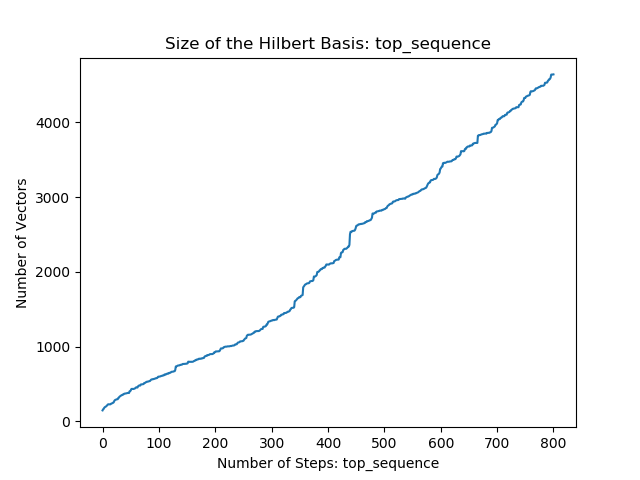
\includegraphics[width=\textwidth]{"4 generators 2 bound A/top_sequence SIZE.png"}
\end{minipage} &
\begin{minipage}{.45\textwidth}
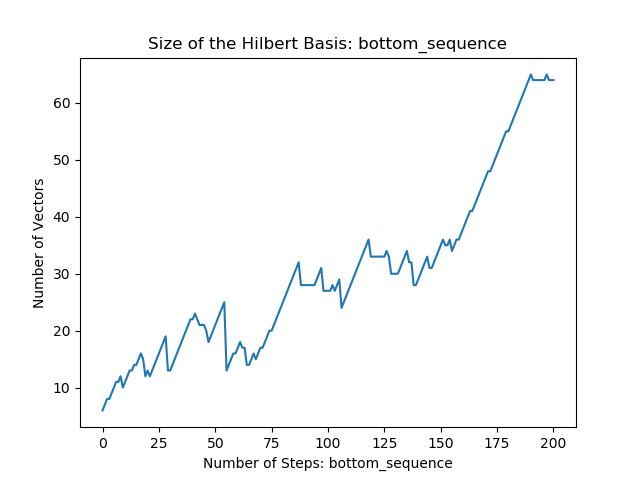
\includegraphics[width=\textwidth]{"4 generators 2 bound A bottomup/bottom_sequence SIZE.png"}
\end{minipage} \\ \\
\hline \\\begin{minipage}{.45\textwidth}
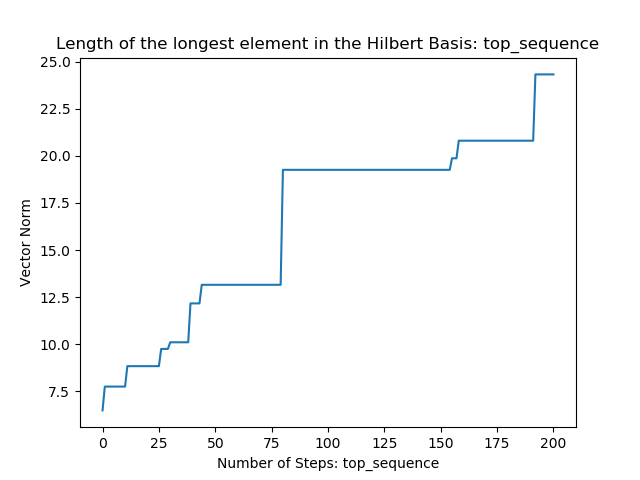
\includegraphics[width=\textwidth]{"4 generators 2 bound A/top_sequence LENGTH.png"}
\end{minipage} &
\begin{minipage}{.45\textwidth}
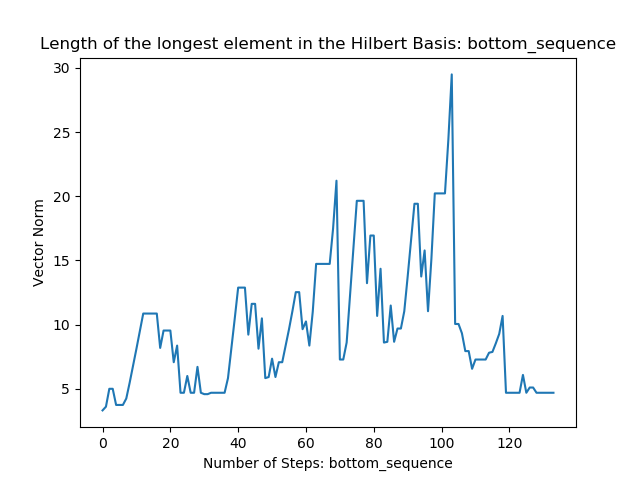
\includegraphics[width=\textwidth]{"4 generators 2 bound A bottomup/bottom_sequence LENGTH.png"}
\end{minipage}
\end{tabular}
\end{document}